% Finnish or English, gives the right language to title page and Finnish enables special chars ä ö å.
\documentclass[a4paper,finnish,12pt]{article}
\bibliographystyle{ieeetr}
\usepackage[T1]{fontenc}
\usepackage[utf8]{inputenc}
\usepackage[finnish]{babel}

\usepackage{mathtools}
\usepackage[lstlisting]{../LaTeX/mcode}
\usepackage{amsfonts,amssymb,amsbsy}
\usepackage{fancyhdr}
\usepackage[a4paper]{geometry}
\usepackage[RGB,ELEC]{../LaTeX/aaltologo}
\usepackage{graphicx}
\usepackage{caption}
\usepackage{subcaption}

\begin{document}

\thispagestyle{empty}

\begin{titlepage}
    \centering
    \vspace*{10\baselineskip}
    \Large
    \bfseries
    AS-0.3100 \\ Automaatio ja systeemitekniikan seminaari \\
    \vspace{\baselineskip}
    \huge
    Osaamisen kehittymisen hallinta \\
    [1.5\baselineskip]
    \normalfont
    \vfill
    \small
    Automaatio- ja systeemitekniikka \\
    \vfill
    Miikka Eloranta \\
    80294A \\[2\baselineskip]
    \textbf{\today} \\[2\baselineskip]
    \vfill
	\AaltoLogoSmall{1}{?}{aaltoPurple}


\end{titlepage}

% DOCUMENT START

\clearpage

\tableofcontents

\clearpage

\section{Johdanto}

Motivaatio lyhyesti.

Tässä työssä keskitytään tieto- ja viestintäteknologian (ICT, information and communications technology) toimialalla työskenteleviin palveluyrityksiin. Vaikka osaltaan tässä raportissa esitetyt käytännöt soveltuvat myös muille toimialoille, ainakin tietyt jaottelut ja keskittyminen osaamisiin on huomioitu vain näiden näkökulmasta.

Toisessa luvussa esitellään tarkemmin motivaatio osaamisten keskitettyyn jatkuvan kehittymisen hallintaan. Kolmannessa luvussa käsitellään tarkemmin osaamisen määritystä, sen mittausperusteita ja jaottelua. Sen lisäksi kolmannessa luvussa esitellään visuaalisesti hyvin havainnollistava T-malli henkilön työroolikohtaisten osaamisten esitykseen. Neljäs luku käsittelee osaamisten kehittymistä, erilaisia kehityksen perusteita ja sen suunnittelua. Viides luku tarjoaa lyhyen katsauksen osaamisten kehittymisen seurantaan ja hallintaan tarkoitetun työkalun tarjoamista mahdollisuuksista.

\clearpage

\section{Motivaatio}

Yritysmaailmassa oman työnsä tehostamiseksi on muiden työntekijöiden lisäksi hyvä tuntea myös kollegoiden osaamisalueet. Pienikokoisissa yrityksissä, pienissä startupeissa tai yksittäisenä yrittäjänä toimiessa tämä on helppoa, koska ihmisiä on vähän tai yksittäisenä yrittäjänä oman osaamisalueen ulkopuoleiseen tekemiseen valitaan juuri siihen aihealueeseen erikoistunut kumppani. Pienyrityksessä kullakin on tarkka vastuualue ja jokainen on osaltaan tärkeä kokonaisuuden kannalta, joten osaamisalueiden tuntemus on oman työnkin kannalta ehdoton vaatimus. Suurissa ja etenkin nopeasti henkilöstömäärällisesti kasvavissa yrityksissä muiden työntekijöiden -- saati näiden kunkin osaamisalueen -- tuntemus on sen sijaan selvästi hankalampaa.

Kollegoiden osaamisten tuntemisen tärkeys korostuu ennen kaikkea asiakaspalveluyrityksiin. Kovassa kilpailutuksessa on osattava kertoa laajemmin koko yrityksen osaamistarjonnasta ja myös olemassa olevien asiakkaiden muuttuviin tarpeisiin on pystyttävä reagoimaan nopeasti -- joko etsimällä tarpeen täyttävä osaaja yrityksen sisältä, rekrytoimalla tai kehittämällä osaamista. Koska kuitenkaan kaikkien yksittäisten asiakkaiden tarpeiden muuttuessa ei osaamista voi välttämättä kehittää tarpeiden mukaan, on osaamisen kehittämistä osattava ennakoida ja valita tärkeimmän kehityssuunnat.

Sen lisäksi, että kollegoiden osaaminen on hyvä tuntea, tulee koko yrityksen osaamistarjonnan olla keskitetysti hallittua, jotta lukumäärällisesti voidaan nopeasti ilmoittaa tietyn osaamisen hallitsevat henkilöt. Monesti asiakkaan kilpailuttaessa palveluyrityksiä tullaan varmistamaan, että tällä on riittävästi asiakkaan tarpeet täyttäviä osaajia.

Teknologiaosaamisten osalta korkean luokan asiantuntijuus ei saisi keskittyä laajalta osin liian pieneen osaan yrityksen henkilöstöä. Vaikka eri työrooleissa asiantuntijuuden syvyys vaihtelee laajalti, ei yksittäinen henkilö saa olla omassa roolissaan korvaamaton. Siinä missä asiakaspalvelija voi vastata laajalti eri teknologioihin tai asiakasympäristöihin liittyvistä perusongelmista, täytyy jollain olla osaamista myös tarkasti kunkin ympäristön arkkitehtuurista. Kuitenkin, jos yksi ja sama henkilö on suunnitellut ja rakentanut kaikkien asiakasympäristöjen tietyt osa-alueet, kostautuu tämä valtavana ongelmana esim. henkilön irtisanoutuessa.

Osaamiset on siis saatava hallitusti jaettua laajemmalle määrälle henkilöstöä pitäen kuitenkin mielessä kunkin työroolin kannalta olennaiset osaamistasot ja alueet. Jotta näitä saadaan hallitusti ja jatkuvasti seurattua ja kehitettyä, on kaikkea henkilöstön osaamista hallittava keskitetysti. Koska kaiken olemassaolevan osaamisen lisäksi sitä on myös kehitettävä, tulee myös kehittämisen olla suunnitelmallista ja suunnitelmia ylläpidettävä tässä yhteydessä yhtä lailla.

\clearpage

\section{Osaaminen -- mitä käytännössä?}

Siinä, missä osaamista voi kasvattaa itse tekemällä tai koulutuksia käymällä, palveluyritysmaailmassa selkeimmät ``merkinnät'' omasta osaamisesta ovat suoritetut sertifioitumiset ja referenssit, jossa asiakkaalta voi varmistaa, että kyseinen henkilö on toiminut tietyssä projektissa tietyssä tehtävässä toteuttaen tiettyjä toimia, tietyillä teknologioilla jne. Sertifioitumiset koostuvat yhdestä tai useammasta suoritetusta testistä, jotka suoritetaan yleensä varsinaisen koulutuksen jälkeen. Käytännössä siis henkilö osoittaa, että on oppinut koulutuksen aihealueen ja ``validoituu'' kyseisen aihealueen osaajaksi.

Varsinainen käytännön osaaminen ei kuitenkaan kartu pelkillä teoriaopinnoilla. Palveluyrityksen valinnassa sertifikaattien ja työkokemuksen lisäksi asiakasyrityksen tulee huomioida sen kumppanit, kumppanuustasot ja olemassa olevat asiakkaat  -- ennen kaikkea lukeutuuko nykyasiakkaisiin saman toimialan yrityksiä \cite{ICT-haasteet}. Vaikka koulutuksessa todennäköisimmin onkin myös käytännön tekemistä, voi sertifikaattitestejä suorittaa myös ilman varsinaiseen koulutukseen osallistumista. Lisäksi voi olla osaajia, jotka eivät ole vielä sertifioituneet tietyn osaamisen osaajiksi -- joko tähän ei ole ollut aikaa tai henkilö ei yksinkertaisesti menesty teoreettisistä testeissä samalla tasolla kuin käytännön osaamisen saralla. Toisaalta on osaamisia, joihin ei yksinkertaisesti voi sertifioitua. Osaaminen pitäisi siis määritellä yleisemmällä tasolla.

Koulutus pelkästään on huono mittari osaamiselle. Saman koulutustaustan ihmiset voivat erota todellisilla osaamisillaan huomattavasti toisistaan. Itsearviointi on kasvattanut valtavasti suosiotaan osaamisen mittaamisessa, vaikkakin myös siinä on huonoja puolia. Kenties suurin syy sen suosioon on nopea tiedonkeruu. Vaikka jokaisella on erilainen näkemys osaamisistaan ja täten arviointiperusteet ovat erilaisia, saadaan tällä ainakin suuntaa-antavaa tietoa osaamisista ja myös epätäydellinen tieto on potentiaalisesti arvokasta. Näiden hyötyjen näkökulmasta katsottuna itsearvioinnin hyödyt ylittävät selkeästi sen huonot puolet. \cite{self-assessment_in_skill_measurement}

Itsearvioiden eroavaisuuksien vuoksi osaamisten arviointeja kannattaa kuitenkin tehdä myös muiden henkilöiden osaamisista. Osaamistasojen oikeellisuuden varmentamiseksi esimiehet voivat arvioida alaistensa osaamisia ja näiden arvioiden ristiriitaisuudessa myös erikseen määritelty osaamiseen paremmin erikoistunut asiantuntija. Käydyt koulutukset, suoritetut sertifikaattitestit ja sertifioitumiset sekä referenssit tehtyihin työtehtäviin antavat osaamiselle pohjaa, mutta osaamisarvio on silti näistä riippumaton.

\subsection{Jaottelu}

Madhavan et. Al tunnisti osaamisisten mittaroinnissa useamman ulottuvuuden. Niin kutsutussa T-mallissa leveys kuvaa osaamisten kokonaismäärää ja korkeus niiden syvyyttä. Mikäli asiantuntijan osaaminen keskittyy esimerkiksi tiettyyn teknologiaan, on hänen osaamisten T-mallissaan kapea, mutta korkea piikki. T-mallia käytetään osaamisten jaottelemiseksi tiettyihin kokonaisuuksiin. \cite{ICT-haasteet}

Tässä ICT-palveluyrityksille tarkoitetussa T-mallissa osaamiset on jaoteltu seuraavasti: \begin{enumerate}
	\item Henkilökohtaiset kyvykkyydet
	%\begin{itemize}
		%\item Kielitaidot
		%\item Tiimityöskentelytaidot
		%\item Paineensietokyky
		%\item \ldots
	%\end{itemize}
	\item Organisaatio- ja toimialakohtaiset osaamiset
	%\begin{itemize}
		%\item Yrityksen kumppanit ja kumppanuustasot
		%\item Kilpailijat
		%\item Asiakkaan edustajien tuntemus
		%\item \ldots
	%\end{itemize}
	\item Ammatilliset ja teknologiaosaamiset.
	%\begin{itemize}
		%\item Microsoft Exchange 2008
		%\item J2EE-ohjelmointi
		%\item Asiakkaan X järjestelmän Y arkkitehtuuri
		%\item \ldots
	%\end{itemize}
\end{enumerate} Kuvassa \ref{fig:Tareas} on esitetty edellä listattujen osaamisalueiden sijainnit T-mallilla. Henkilökohtaisiin kyvykkyyksiin määritellään kaikki henkilön omaan käyttäytymiseen, muiden kanssa kommunikointiin ja kyvykkyyteen toimia tietyissä rooleissa. Näihin kuuluvat muun muassa kielitaidot, tiimityöskentelytaidot tai paineensietokyky. Organisaatio- ja toimialakohtaisiin osaamisiin taas määritelään mm. kaikki yrityksen käytäntöihin liittyvät osaamiset, kilpailijat, kumppanit ja kumppanuustasot, sekä asiakkaan edustajien tuntemus. Viimeisenä ammatillisiin ja teknologiaosaamisiin liittyy kaikki eri teknologioihin, ohjelmointikieliin ja -kehitykseen, asiakkaiden järjestelmien arkkitehtuureihin yms. liittyvät osaamiset. T-malli on valittu, koska osa-alueita on kolme ja kukin sen osio kuvaa yhtä osa-alueista.

\begin{figure}[!ht]
	\centering
	\begin{subfigure}[t]{0.45\textwidth}
		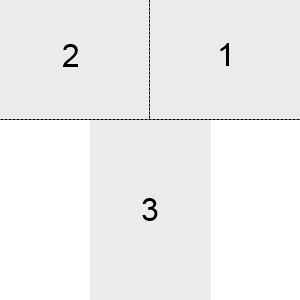
\includegraphics[width=\textwidth]{T_areas.png}
		\caption{Käytetyt osaamisaluejaot ICT-palveluyritykselle.}
		\label{fig:Tareas}
	\end{subfigure}
	\hfill
	\begin{subfigure}[t]{0.45\textwidth}
		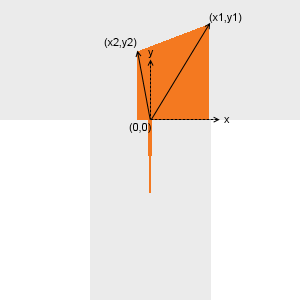
\includegraphics[width=\textwidth]{T_drawing_logics.png}
		\caption{Piirtologiikka valitulle työroolille.}
		\label{fig:Tlogics}
	\end{subfigure}
	\caption{T-mallin osaamisalueet ja piirtologiikka.}
\end{figure}

Koska kullakin työroolilla kaivataan erityyppisiä osaajia, T-mallia piirrettäessä sen kukin haara skaalataan rooliin vaadittavien osaamisten mukaisesti. T-mallin yläosa piirretään käyttäen yhtälöparin %\eqref{Tlogics_optim} ja \eqref{Tlogics} mukaisella logiikalla, joka on myös esitetty kuvassa \ref{fig:Tlogics}. Taustalla näkyvä harmaa T on valitun työroolin ``optimi-T,'' joka pitää sisällään kaikki työroolin osaamiset. Harmaa T-malli skaalataan osaamisten lukumäärien mukaisesti symmetriseksi yhtälön \eqref{Tscaleconstants} mukaisesti ja näin saatuja skaalauskertoimia käytetään henkilön T-mallin piirrossa. Yhtälön \eqref{Tscaleconstants} muuttuja $A_1$ on skaalauskerroin henkilökohtaisten kyvykkyyksien leveydelle, $A_2$ vastaavasti organisaatio- ja toimialakohtaisten osaamisten leveyksille ja $B_1$ sekä $B_2$ vastaavat korkeusskaalaimet.
\begin{equation}
\begin{cases}
A_i = \frac{1}{n_1} \\
B_i = \frac{1}{5} \\
\end{cases} \\ , i \in [1,2]
\label{Tscaleconstants}
\end{equation} skaalauskertoimia, jossa $A_i$ on osaamisalueen $i$ skaalauskerroin leveydelle ja $n_i$ vastaavan alueen osaamisten kokonaislukumäärä. $B_i$ on vastaavasti korkeuden skaalauskerroin, joka on kaikille $1/5$, koska osaamistasoja on tässä määritelty viisi kappaletta ja korkeus määritetään henkilölle määriteltyjen osaamisten tasojen keskiarvona.

Osaamisalueessa 3 osaamisen leveys kuvaa osaamisten lukumäärää ``vähintään tasolla x.'' Harmaan alueen leveys määrittyy osaamisten lukumäärästä kaksinkertaisena, sillä tähän alueeseen piirrettävä kuvaaja peilataan $y$-akselin ympäri. Alaspäin mentäessä tasot kasvavat tasaisin väliajoin jolloin T-mallin ``jalasta'' tulee alaspäin porrastettu. Täten jokaisessa ``portaassa'' on vähintään yhtä paljon osaamisia, eli se on vähintään yhtä leveä kuin seuraavassa liikkuessa alaspäin. Koska 3. osaamisalueessa osaamistasokohtainen korkeus on vakio, jokaisella voi tässä käyttää alueen korkeuteen suoraan verrannollista skalaarikerrointa $B_3$, joka vastaa täysin yhtälön \eqref{Tscaleconstants} kerrointa $B_i$. Näin ollen kulmapisteet osaamisalueelle 3 saadaa yhtälöistä
\begin{equation}
\begin{cases}
A_i = \pm \sum_{o \in O_i} \frac{O_i}{n_i} = \frac{1}{n_i} \pm \sum_{o \in O_i} o \\
B_i = \frac{1}{5}
\end{cases} \\ i = 3.
\label{Tscaleconstants3}
\end{equation} 

Käyttäen kertoimia yhtälöistä \eqref{Tscaleconstants} ja \eqref{Tscaleconstants3} saadaan henkilölle määriteltyä kuvan \ref{fig:Tlogics} mukaiset osaamisalueiden 1 ja 2 pisteet $(x_1, y_1)$, $(x_2, y_2)$, $(x_3^1, y_3^1$) ja $(x_3^2, y_3^2)$ yhtälöillä
\begin{equation}
\begin{cases}
x_i = (-1)^{i-1} A_i \cdot \frac{n_{io}}{n_i} = \frac{A_i}{n_i} n_{io} \\
y_i = B_i \cdot \sum_{k \in O_i} \frac{O_k}{n_i} = \frac{B_i}{n_i} \sum_{o \in O_i} o, \\
\end{cases}
\end{equation} jossa $n_{io}$ on henkilön osaamisten lukumäärä osaamisalueessa $i$, $O_i$ kattaa henkilölle määritettyjen osaamisten tasot osaamisalueessa $i$.

Vaikka T-malli havainnollistaakin omalta osaltaan henkilön osaamisprofiilia ja sitä, mihin osa-alueeseen se keskittyy -- tai keskittyykö mihinkään yksittäiseen -- on siinä myös puutteita. Jotta T-mallista saisi paremman kuvan henkilön osaamisista, tulisi kussakin osaamisalueessa olla suuruusluokaltaan yhtä paljon osaamisia. Kuitenkin teknologiat kehittyvät jatkuvasti, ja eri versioiden osaaminen on eriytettävä toisistaan, jotta näitä voidaan hyödyntää jatkossa. Tämän lisäksi eri teknologioiden osaaminen itsessään ei mittarina riitä, vaan kunkin asiakasympäristön arkkitehtuurin tuntemus olisi hyvä pitää omana osaamisenaan.

Tästä johtuen teknologia- ja ammatillisia osaamisia tulee T-malliin etenkin ICT-palveluyrityksissä huomattavasti enemmän kuin henkilökohtaisia kyvykkyyksiä tai organisaatio- ja toimialakohtaisia osaamisia. Vaikka eri osaamiset sidotaankin T-malliin eri rooleissa, tulee tällä alalla lähes kaikille rooleille valtaosaksi teknologiaosaamisia. T-mallissa 3. osaamisalueen kuvaajan leventäminen vaatii siis huomattavasti enemmän uusia osaamisia kuin osaamisalueiden 1 tai 2. Lisäksi osaaminen suuremmassa määrässä osaamisia aiheuttaa todennäköisesti tämän osa-alueen osaamisten syvyyden heikentymistä. Tästä syystä osaamisalueen 3 piirtologiikka eroaakin muista alueista, eikä tässä käytetä osaamisten keskiarvoa, jotta se visualisoisi osaamisten laajuutta paremmin.

\clearpage

\section{Jatkuva kehittyminen}

Osaamisen kehittyminen on jatkuva prosessi. Kun teknologiat, prosessit ja menetelmät kehittyvät, asiakkaat haluavat siirtyä niihin. Tämän tarpeen seurauksena palveluyrityksen asiantuntijat kouluttautuvat niihin, osaaminen näihin kasvaa ja tarpeet saadaan täytettyä. Koska kuitenkin tämän seurauksena teknologian osaajien määrä ja tietoisuus siitä maailmalla kasvaa, myös teknologian kehittäjä saa lisää mahdollisuuksia jatkokehittää sitä. Melko ylätason kuvaus tästä jatkuvasta prosessista on esitetty kuvassa \ref{fig:perusympyra}. Luonnollisesti myös palveluyrityksessä henkilöstö muuttuu ja näistä aiheutuu mahdollisisti kehitystarpeita tai niiden täyttymisiä. Ne on esitetty kuvassa katkoviivalla. Vaikka tarpeita uusien teknologioiden osaamiseen ei suoraan olemassaolevilta asiakkailta tulisikaan, palveluyritysten kilpailun vuoksi yriyksen on pidettävä oma osaamisensa jatkuvasti ajan tasalla säilyttääkseen kilpailukykynsä.

\begin{figure}[ht]
\centering
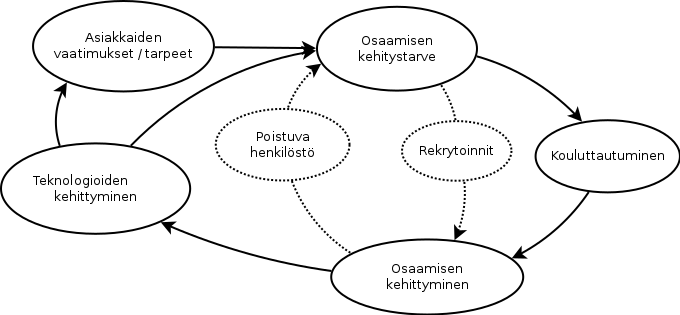
\includegraphics[scale=0.5]{knowledge_circle.png}
\caption{Osaamisen jatkuva kehittäminen}
\label{fig:perusympyra}
\end{figure}

Uudet teknologiat, kasvava yritys, vitusti pilvee Kalliosta

\subsection{Kehittymisen suunnittelu}

Koko organisaation kehityssuunnat määrittyvät yksilöiden kautta. Vaikka organisaatiolla olisikin tietyt tavoitteet kehityssuunniksi, sen toteutuminen on riippuvaista siitä, onko osaamisen kehitystä hankkiva henkilökunta motivoitunutta. Tästä syystä henkilöstön itsensä tulee saada olla vaikuttamassa oman henkilökohtaisen koulutussuunnitelmansa tekoon. Kehittymisen suunnittelu onkin jaoteltu kahteen eri suuntaan: koulutussuunnitteluun sekä organisaation tavoitteisiin. Koulutussuunnittelussa henkilö saa itse asettaa itselleen ylätason tavoitteet, millaisia koulutuksia hän suunnittelee käyvänsä. Koulutussuunnitelma käydään läpi lähiesimiehen kanssa, joka voi viime kädessä ilmoittaa, mikäli suunnitelmaa on esim. budjetäärisistä syistä korjattava.

Organisaation tavoiteasetannassa johtoryhmä tekee päätökset yrityksen pääasiallisista tavoitteellisista kehityssuunnista. Asiantuntijoiden itselleen asettamia koulutussuunnitelmia käytetään tässä osviittana siitä, millaista koulutusta voitaisiin motivoidusti asettaa henkilöstölle, mutta kehittyvät ja uudet teknologiat sekä mahdolliset asiakastarpeet, joihin kehittyminen on välttämätöntä, määrittävät lopulliset tavoitteet. Johtoryhmän asettamat tavoitteet laskeutuvat asiantuntijoille portaittain siten, että kukin esimies saatuaan tavoitteen tekee päätöksen, millä tavalla hän voi kyseisen tavoitteen toteutumista edesauttaa ja määrittää siitä tavoitteen omille alaisilleen -- tai osalle heistä -- hieman konkreettisemmalla tasolla. Lopulta koko tavoitepolkua voidaan tarkastella johtoryhmän asetannasta asiantuntijoille määriteltyihin tavoitteisiin ja tehdä viimeisiä korjauksia, jos nämä eivät kata alkuperäisen tavoitteen vaatimuksia. Ylätason esimerkki tälläisestä tavoiteasetannasta on esitetty kuvassa \ref{fig:tavoitesample}. Tästä nähdään kuinka tavoite tarkentuu hieman jokaisella organisaatioportaalla.

\begin{figure}[hb]
\centering
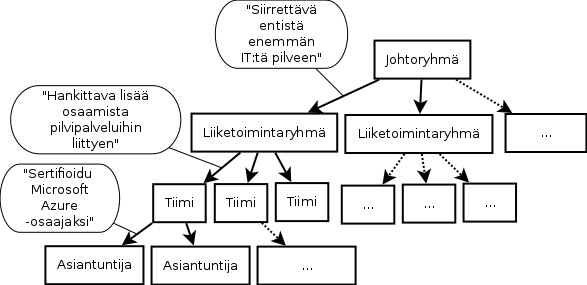
\includegraphics[width=1\textwidth]{tavoitesample.png}
\caption{Esimerkki tavoiteasetannasta, joka kulkee johtoryhmästä organisaatioportaiden kautta asiantuntijalle konkreettisemmaksi tavoitteeksi.}
\label{fig:tavoitesample}
\end{figure}

\subsection{Urapolut}

Jotta työntekijöitä saataisiin motivoitua kehittämään itseään, tulee heidän urakehittymismahdollisuutensa olla selkeästi tiedossa. Koska jokaiselle roolille on asetettu konkreettiset tavoitteet kullekin roolitasolle 1-5, voidaan nämä visualisoida selvästi ns. urapolkunäkymänä. Urapolkunäkymästä on esitetty esimerkki testitunnukselta kuvassa \ref{fig:urapolkuspiderweb}. Kuvassa oranssilla on kuvattu työrooli, johon työntekijä varsinaisesti on määritelty ja harmaalla roolit, joista vaatimuksia on täyttynyt prosentuaalisesti esityksen mukainen täyttömäärä. Koska rooleissa on tasot 1-5 ja kullakin tasolla omat vaatimuksensa, ei käytännössä tasolla voi nousta ylöspäin, jos alemman tason vaatimukset eivät täyty. Kuitenkin nämä on täytetty erikseen, jotta henkilö itse näkee, kuinka pitkälle hän alemman tason vaatimukset täyttämällä voisi edetä.

\begin{figure}[ht]
\centering
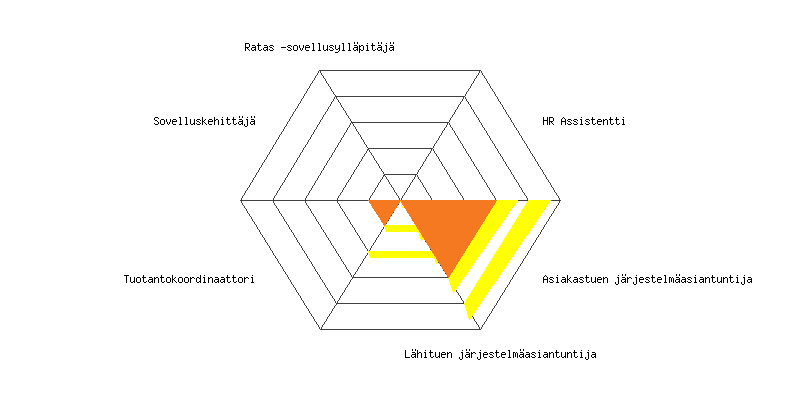
\includegraphics[width=1\textwidth]{urapolkuPlot_tst_usr.png}
\caption{Esimerkki testihenkilön urapolkunäkymästä, jossa tämänhetkiset roolit on merkitty oranssilla ja muiden roolien vaatimusten täyttymisaste harmaalla.}
\label{fig:urapolkuspiderweb}
\end{figure}

\clearpage

\section{Keskitetty hallinta}

Keskitetyssä hallinnassa koko yrityksen osaamisia ylläpidetään samassa järjestelmässä. Kun osaamisista suoritetaan itsearviointeja, esimiesarviointeja ja mahdollisia erityisasiantuntijan arviointeja, saadaan osaamisten todellisesta tasosta kattavampi kuva. Kun kaikki kerätty data osaamisten, näiden kehittymisten, tavoiteasetantojen ja näiden toteutumien osalta on ylläpidetty yhdessä paikassa, voidaan datan perusteella tuottaa erilaisia raportteja. Raporttien perusteella jatkuva seuranta on myös mahdollista. 

Keskitetyn hallinnan ja sen raportoinnin toimivuuden varmentamiseksi kunkin työntekijän on itse vastattava omien tietojensa ajantasaisuudesta ja jatkuvasta päivittämisestä. Mikäli osa henkilöstöstä ei pidä tietojaan ajan tasalla, ei myöskään järjestelmästä saatavaa informaatiota voi pitää luotettavana. Jotta järjestelmästä saataviin raportteihin voisi luottaa, on jokaisen sitouduttava omien tietojensa ylläpitoon -- muuten koko yritys näyttää markkinassa ja asiakkaiden silmissä heikommalta.

\begin{itemize}
\item Järjestelmä yleisläpinä?
\item Kehittymisen suunnittelu ja toteutumisen seuranta
\item CV-generointi
\end{itemize}

\subsection{Hyödyt}

Pidemmällä tähtäimellä osaamisten keskitetyn hallinnan hyödyntämistä voi laajentaa moniin tarkoituksiin. Tavoiteasetantojen toteutumien seuranta havainnollistaa organisaation johdolle sitä, olivatko annetut tavoitteet toteuttamiskelpoisia tai onko niiden toteutumatta jäämiseen ollut jokin selvä syy, johon pitää puuttua. Kuvan \ref{fig:tavoitesample} mukaisilla tavoiteasetannoilla myös yksittäisille asiantuntijoille asetettujen tavoitteiden toteumat voi linkittää suurempaan kokonaisuuteen, ja tavoitteiden toteutuessa nämä liittää suoraan tuloskortille -- sitoen henkilötön tulospalkkiot niihin. Vaikka tuloskortin tavoitteet eivät tällä tapaa suoraan henkilötölle konkretisoituisikaan, tavoitteen kohdeympäristöä voi hyödyntää tavoitteiden toteutumisiin tai niiden toteutumatta jäämisiin puuttuessa.

Kun osaamiset, kehittymiset, suoritetut sertifioitumiset ja mahdollisesti esimerkiksi asiakasreferenssit on keskitetty yhteen järjestelmään, voi tätä hyödyntää paljon myös muiden järjestelmien yhteydessä. Koska jokaiselle henkilölle määritellyt taidot ja osaamiset on keskitetty, integroimalla tämän henkilöstönhallintajärjestelmään voidaan raportoinnin kautta luoda esimerkiksi myynnillisiä tai roolikohtaisia CV:itä.

\clearpage

\section{Yhteenveto ja johtopäätökset}

Kai tää ois ihan jeppis?

\clearpage

\clearpage

%% Lähdeluettelo
\addcontentsline{toc}{section}{Viitteet}
\bibliography{refet}

\appendix


\end{document}
